\documentclass[12pt,a4paper]{report}
\usepackage[utf8]{inputenc} % this is needed for umlauts
\usepackage[ngerman]{babel} % this is needed for umlauts
\usepackage[T1]{fontenc}    % this is needed for correct output of umlauts in pdf

\usepackage{ucs}
\usepackage{amsmath}
\usepackage{amsfonts}
\usepackage{amssymb}
\usepackage{graphicx}

\usepackage{hyperref}
\usepackage{csquotes}
\usepackage{appendix}
\usepackage{pdfpages}
\usepackage{float}

\delimitershortfall-1sp
\newcommand\abs[1]{\left|#1\right|}

\usepackage[weather]{ifsym}

\begin{document}

\newcommand \GruppeA {henrilibre}

	\tableofcontents
	
	\newpage
	\setcounter{chapter}{-1}
\chapter{Vorwort}
	Dieses Dokument findest du auf github.com unter: \href{https://github.com/henri-libre/analysis1}{https://github.com/henri-libre/analysis1}. Du darfst das Dokument nutzen, erweitern und verbreiten. Maintainer des Dokumentes erreichst du entweder dort oder per E-Mail an \href{analysis1istgeil@nanooq.org}{analysis1istgeil@nanooq.org}. Für die Korrektheit des Dokumentes ist entweder keiner oder du verantwortlich. Die URL der Veranstaltung an sich lautet: \href{https://analysis3.wordpress.com/analysis-i-ws-1516/uebungen-zu-analysis-i-wise-1516/}{https://analysis3.wordpress.com/analysis-i-ws-1516/uebungen-zu-analysis-i-wise-1516/}
	
\chapter{Übungsblatt 1}
	
	Das entsprechende Übungsblatt befindet sich im Anhang \ref{uebungsblatt1} \footnote{\href{https://analysis3.files.wordpress.com/2015/08/blatt1.pdf}{https://analysis3.files.wordpress.com/2015/08/blatt1.pdf}}.

\newpage		
\section{Übungsblatt1, Aufgabe 1: Vollständige Induktion, 4 Punkte, \GruppeA}
	
	\begin{enumerate}
	\item Z.~z.: $5^n - 1 | 4 $ 
		\begin{itemize}
			\item Induktionsanfang:
			\begin{flalign*}
				n_1 = 1: ~~& 5^1 - 1 = 4 ~~ \checkmark &\\
				n_2 = 2: ~~& 5^2 - 1 = 24~~ \checkmark &\\
				n_3 = 3: ~~& 5^3 - 1 = 124~~ \checkmark
			\end{flalign*}
			\item Induktionsvoraussetzung:
			\begin{flalign*}
				(5^n -1) | 4 &&
			\end{flalign*}
			\item Induktionsschritt:
			\begin{flalign*}
				n \mapsto n+1: ~~ & 5^{n+1}-1 & \\ 
				= & (5 \cdot 5^n)-1 & \\
				= & (4 \cdot 5^n + 5^n) -1 & \\
				= & (4 \cdot 5^n) + (5^n -1)
			\end{flalign*}
			Erster Term ist durch 4 teilbar. Zweiter Term ist gleich unserer Induktionsvoraussetzung.  
		\end{itemize}
	\newpage
	\item Z.~z.: $ 3^{2^n}-1|2^{n+2} $ 
		\begin{itemize}
			\item Induktionsanfang:
			\begin{flalign*}
				n_1 = 1: ~~& 3^{2^1} - 1 | 2^{1+2} \Leftrightarrow 8 | 8 ~~ \checkmark & \\
				n_2 = 2: ~~& 3^{2^2} - 1 | 2^{2+2} \Leftrightarrow 80 | 16 ~~ \checkmark & \\
				n_3 = 3: ~~& 3^{2^3} - 1 | 2^{3+2} \Leftrightarrow 6560 | 32 ~~ \checkmark
			\end{flalign*}
			\item Induktionsvoraussetzung:
			\begin{flalign*}
				3^{2^n} - 1 | 2^{n+2} &&
			\end{flalign*}
			\item Induktionsschritt:
			\begin{flalign*}
				n \mapsto n+1: ~~ & 3^{2^{n+1}} -1 & \\
				 \overset{\text{aus Klammer ziehen}}{=} & (3^{2^n})^2 -1 &\\ 
				 \overset{\text{3. Binomische Formel}}{=} & (3^{2^n}-1)(3^{2^n}+1) 
			\end{flalign*}

			Erster Term ist die Induktionsvoraussetzung. Der zweite Term ist im Detail unwichtig, wegen der Multiplikation.
		\end{itemize}
	\item Z.~z.: Für Menge $M$ mit $|M| = n \Rightarrow |P(M)|=2^n$
		\begin{itemize}
			\item Induktionsvoraussetzung:
			$ n=1: $ Sei $M=\{n\}$. Dann ist $P(M)=\{\varnothing,\{a\}\} \rightarrow |P(M)|=2^1$.
			\item Induktionsschritt:\\
			Dann sei $M^*=\{a_1,\dots, a_n\}$.\\
			Dann gilt laut Induktionsvoraussetzung: $|P(M^*)=2^n|$.
			\\Nun gilt\footnote{$P(M) \setminus P(M^*)$ muss disjunkt sein, weil: Wenn A, B disjunkt, dann $ A \cap B = \varnothing$.} $P(M) \setminus P(M^*) = \{T \cup \{a_{n+1}\} | T \in P(M^*)\} \\
			\Rightarrow |P(M)|=2|P(M^*)|=2\cdot 2^n= 2^{n+1}$
			\item Erklärung:\\
			Es sei $ P(m^*) = \{\varnothing\}, \{a_1\}, \{a_2\}, \{a_1,a_2\}$. Wenn nun $ \{a_3\} $ hinzugefügt wird, ist $ P(m) = P(m^*) \cup \{a_{3}\} = \{\varnothing\}, \{a_1\}, \{a_2\}, \{a_1,a_2\},\\
			\{a_3\}, \{a_1,a_3\}, \{a_2,a_3\}, \{a_1,a_2,a_3\} $.
		\end{itemize}
	\end{enumerate}

\newpage
\section{Übungsblatt 1, Aufgabe 2: Indirekter Beweis, 4 Punkte, \GruppeA}
		
	Zeige zunächst: $ (1+k) \leq 2^k $ ~~ $ \forall ~ k \in N$
	\begin{itemize}
		\item Induktionsanfang:
		\begin{flalign*} 
		k_1 = 1: ~~ & 1 + 1 \leq 2^1 \Leftrightarrow 2 \leq 2 ~~ \checkmark & \\
		k_2 = 2: ~~ & 1 + 2 \leq 2^2 \Leftrightarrow 3 \leq 4 ~~ \checkmark & \\
		k_3 = 3: ~~ & 1 + 3 \leq 2^3 \Leftrightarrow 4 \leq 8 ~~ \checkmark
		\end{flalign*}
		\item Induktionsvoraussetzung:
		\begin{flalign*}
			(1+k) \leq 2^k ~~ \forall ~ k \in N &&
		\end{flalign*}
		\item Induktionsschritt:
			\begin{flalign*}
			k \mapsto k+1: ~~  1+(k+1) &\leq 2^{k +1} & \\
			\Leftrightarrow (2+k) &\leq 2 \cdot 2^k & \\
			\Leftrightarrow \frac{2+k}{2} &\leq (1+k) \leq 2^k
			\end{flalign*}
			Der erste Term ist immer kleiner als die linke Seite der Induktionsvoraussetzung.
		\end{itemize}

	Exkurs \enquote{Indirekter Beweis}: $(A \Rightarrow B) \Leftrightarrow (\neg B \Rightarrow \neg A)$:

	\begin{table}[H]
		\center
		\begin{tabular}{c | c | c | c | c }
			\# & A & B & A $\Rightarrow B $ & $ \neg B \Rightarrow \neg A $ \\
			\hline
			1 & 0 & 0 & 1 & 1 \\
			2 & 0 & 1 & 1 & 1 \\
			3 & 1 & 0 & 0 & 0 \\
			4 & 1 & 1 & 1 & 1 \\
		\end{tabular}
		\caption{In der dritten Zeile steht der Indirekter Beweis}
	\end{table}
	
	Indirekter Beweis: Z.~z.: Für $ a_1, \ldots, a_n \text{ mit } n \in N$ gilt:\\
	\begin{align*}
	\prod^{n}_{i=1}(1+a_i) > 2^n\text{, so folgt} \sum^{n}_{i=1}a_i > n &&
	\end{align*}
	Eigentlich sieht das so schöner aus:
	\begin{align*}
	n < \sum^{n}_{i=1}a_i < 2^n < \prod^{n}_{i=1}(1+a_i)&&
	\end{align*}	
	
	\begin{itemize}
		\item \enquote{Anfang}. Einfach mal durchrechnen:
		\begin{flalign*}
			n_1 = 1: ~~ & 1 < 1 < 2^1 < (1 + 1) ~~ \text{\Lightning} & \\
			n_2 = 2: ~~ & 2 < 1+2 < 2^2 < (1+1)(1+2) ~~ \checkmark & \\
			n_3 = 3: ~~ & 3 < 1+2+3 < 2^3 < (1+1)(1+2)(1+3) ~~ \checkmark &
		\end{flalign*}
		\item \enquote{Voraussetzung}, zu zeigen:
			\begin{flalign*}
			n < \sum^{n}_{i=1}a_i < 2^n < \prod^{n}_{i=1}(1+a_i) &&	
			\end{flalign*}
		\item Indirekter Beweis:
			\begin{flalign*}
			& \prod^{n}_{i=1}(1+a_i) = (1+a_1) \cdot \ldots \cdot (1+a_n) & \\
			& \text{jeder Term kleiner als} & \\
			& \leq 2^{a_1} \cdot \ldots \cdot 2^{a_n} = 2^{\sum_{i=1}^{n}a_i} &\\
			& \overset{\text{vorhin bewiesen}}{\leq} 2^n & \\ 
			\end{flalign*}
	\end{itemize}
\newpage
\section{Übungsblatt 1, Aufgabe 3: Vollständige Induktion, 4 Punkte, \GruppeA}

	\begin{enumerate}
		\item Z.~z. dass das Brett mit \enquote{L}-förmigen Kartonstücken überdecken.
		\begin{itemize}
			\item Iinduktionsanfang:
				\begin{table}[H]
					\centering
					\begin{tabular}{|c|c|c|c|}
						\hline
						~~&~~&~~&~~\\
						\hline
						&&&\\
						\hline
						&&&\\
						\hline
						&&&\\
						\hline
					\end{tabular}
					\caption{Schachbrett mit der Seitenläge $2^n$}
				\end{table}
			\item Induktionsvoraussetzung:\\
			$n=1: 2 \times 2 \rightsquigarrow$ \enquote{L}-förmiges Kartonstückchen $\Rightarrow$ Vollständige Überdeckung.
			
			\item Induktionsschritt:\\
			$n\mapsto n+1$: Wir nehmen von einem Schachbrett mit Seitenlänge $2^{n+1}$ ein Feld weg und teilen es in 4 Schachbretter mit der Seitenlänge $2^n$ auf:
			\begin{table}[H]
				\centering
				\begin{tabular}{|c|c||c|c|}
					\hline
					2 & 2 & 1 & X \\
					\hline
					2 & 2 & 1 & 1 \\
					\hline
					\hline
					3 & 3 & 4 & 4 \\
					\hline
					3 & 3 & 4 & 4 \\
					\hline
				\end{tabular}
				\caption{Schachbrett mit der Seitenläge $2^{n+1} $, das weggenommene Feld sei X}
			\end{table}
			Sei das weggenommene Feld ohne Beschränkung der Allgemeinheit oben rechts aus 1. Dann können wir laut Induktionsvoraussetzung das Feld 1 vollständig überdecken. Genauso können wir dies mit den Feldern 2, 3 und 4 bis auf ein Feld überdecken. Diese drei Felder werden so angeordnet:
			
			\begin{table}[H]
				\centering
				\begin{tabular}{|c|c||c|c|}
					\hline
					2 & 2 & 1 & X \\
					\hline
					2 & L & 1 & 1 \\
					\hline
					\hline
					3 & L & L & 4 \\
					\hline
					3 & 3 & 4 & 4 \\
					\hline
				\end{tabular}
				\caption{}
			\end{table}
			
			Dann können wir diese drei Felder auch überdecken. Dann ist das gesamte Brett mit Ausnahme des weggenommenen Feldes vollständig überdeckt. $ \square $
		\end{itemize}
	\item Aus dem ersten Aufgabenteil folgt nicht, dass der Beweis für diesen Aufgabenteil. Viel mehr ist der erste Teil ein Spezialfall von diesem Aufgabenteil.\\
	Z.~z.: $ 3|2^{2n}-1$
	\begin{itemize}
		\item Iinduktionsanfang:
		\begin{flalign*}
			n_1 = 1:~~ & 2^{2\cdot 1} - 1 = 3  ~~\checkmark &\\
			n_2 = 2:~~ & 2^{2\cdot 2} - 1 = 15 ~~\checkmark &\\
			n_3 = 3:~~ & 2^{2\cdot 3} - 1 = 63 ~~\checkmark &
		\end{flalign*}
		\item Induktionsvoraussetzung:
		\begin{flalign*}
			3|2^{2n}-1 &&
		\end{flalign*}
		\item Induktionsschritt:
		\begin{flalign*}
			n \mapsto n+1: ~~ & 2^{2(n+1)} - 1 & \\
			& = 2^{2n+2} - 1 & \\
			& = (2^{2n} - 1 + 1) \cdot 4 - 1 & \\
			& = (2^{2n} - 1) \cdot 4 + 1 \cdot 4 - 1 & \\
			& = 4(2^{2n} - 1) + 3
		\end{flalign*}
		Der letzte Term ist durch 3 teilbar.  Die Multiplikation am Anfang ist ein Vierfaches der Induktionsvoraussetzung. Die Induktionsvoraussetzung selber ist durch 3 teilbar. Also ist auch die Multiplikation durch 3 teilbar. Damit ist die ganze Formel durch 3 teilbar.
	\end{itemize}
	\end{enumerate}

\newpage
\section{Übungsblatt 1, Aufgabe 4: Vollständige Induktion, 4 Punkte, \GruppeA}
Der Fehler in dem Induktionsverwis liegt im Folgenden: Innerhalb des Induktionsschrittes nimmt die Induktionan, dass die Induktionsannahme gleich der Behauptung, also wahr, ist. Dieser Schritt ist jedoch fehlerhaft, da nie bewiesen wurde, on jede Aussage wahr ist. Da man von einer falschen Aussage auf sowohl wahre als auch falsche Aussage schließen kann, fehlt daher ein Berweis, dass die Induktionsanname wahr ist. Ein Gegenbeweis wäre z.~B. für $n=2$.

\newpage
\section{Musterlösung}

Stand 2015-10-29: Noch nicht bekannt gegeben



\chapter{Übungsblatt 2}

	Das entsprechende Übungsblatt befindet sich im Anhang \ref{uebungsblatt2} \footnote{\href{https://analysis3.files.wordpress.com/2015/08/blatt-2.pdf}{https://analysis3.files.wordpress.com/2015/08/blatt-21.pdf}}.
	
	\newpage		
	\section{Übungsblatt 2, Aufgabe 1: Konvergenz von Reihen, 4 Punkte, \GruppeA}
	
	\begin{enumerate}
		\item Z.z. $ \forall ~ n \in N \text{, gilt }\sum^{n}_{k=1} \frac{1}{k(k+1)} = 1 - \frac{1}{n+1} $	\begin{itemize}
			\item Induktionsanfang:
			\begin{flalign*}
			n = 1: ~~  \frac{1}{1(1+1)} = 1 - \frac{1}{1+1} & \Leftrightarrow \frac{1}{2} = \frac{1}{2} ~~~ \checkmark &  \\
			n = 2: ~~  \frac{1}{2(2+1)} = 1 - \frac{1}{2+1} & \Leftrightarrow \frac{2}{3} = \frac{2}{3} ~~ \checkmark & 
			\end{flalign*}
			\item Induktionsvoraussetzung:
			\begin{flalign*}
			\sum^{n}_{k=1} \frac{1}{k(k+1)} & = 1 - \frac{1}{(n+1)}
			\end{flalign*}
			\item Induktionsschritt:
			\begin{flalign*}
			n \mapsto n+1: ~~ & \sum^{n+1}_{k=1} \frac{1}{k(k+1)} = 1 - \frac{1}{((n+1)+1)} = 1 - \frac{1}{(n+2)} & \\
			& \overset{\text{I.V.}}{=} 1 - \frac{1}{n+1} + \frac{1}{(n+1)(n+2)} & \\
			& = \frac{(n+1)(n+2)-(n+2)+1}{(n+1)(n+2)} & \\
			& = \frac{(n+1)(n+2)-n-1}{(n+1)(n+2)} & \\
			& = \frac{(n+1)(n+2)-(n+1)}{(n+1)(n+2)} & \\
			& = \frac{(n+1)(n+2)}{(n+1)(n+2)} - \frac{(n+1)}{(n+1)(n+2)} & \\
			& = 1 - \frac{1}{(n+2)} & \square
			\end{flalign*}
		\end{itemize}
		\newpage
		\item Z.z. $ \forall ~ n \in N \text{, gilt } \sum^{n}_{k=1} k^3 = \frac{n^2(n+1)^2}{4} $
		\begin{itemize}
			\item Induktionsanfang:
			\begin{flalign*}
			\sum^{n}_{k=1} k^3 & = 1 - \frac{n^2(n+1)^2}{4} & \\
			n = 1: ~~  \sum^{n}_{k=1} k^3 & = 1 - \frac{n^2(n+1)^2}{4} ~~ \checkmark & \\
			\end{flalign*}
			\item Induktionsvoraussetzung:
			\begin{flalign*}
			\sum^{n}_{k=1} k^3 & = 1 - \frac{n^2(n+1)^2}{4} & \\
			\end{flalign*}
			\item Induktionsschritt:
			\begin{flalign*}
			n \mapsto n+1: ~~ & \sum^{n+1}_{k=1} k^3 = 1 - \frac{(n+1)^2((n+1)+1)^2}{4} & \\
			& \overset{\text{rechten Term ausrechnen}}{=} \frac{n^4+6n^3+14n^2+12n+4}{4} & \\
			& \overset{\text{I.V.}}{=} \frac{n^2(n+1)^2}{4} + (n+1)^3 & \\
			& \overset{\text{ausrechnen}}{=} \frac{n^4+6n^3+14n^2+12n+4}{4} & \square
			\end{flalign*}
		\end{itemize}
	\end{enumerate}
	
	\newpage
	\section{Übungsblatt 2, Aufgabe 2: Kombinatorik, 4 Punkte, \GruppeA}
	\begin{flalign*}
		n = 3: ~~ & (1,1,1) & \Rightarrow p(3) = 1 \\
		n = 4: ~~ & (2,1,1), (1,1,2), (1,2,1) & \Rightarrow p(4) = 3 \\
		n = 5: ~~ & (3,1,1), (1,1,3), (1,3,1), & \Rightarrow p(5) = 6 \\
		& (2,1,2), (2,2,1), (1,2,2) & \\
		n = 6: ~~ & (4,1,1), (1,4,1), (1,1,4), & \Rightarrow p(6) = 10 \\
		& (3,2,1), (3,1,2), (2,1,3), (2,3,1), (1,2,3), (1,3,2), & \\
		& (2,2,2) & \\
		n = 7: ~~ & (5,1,1), (1,5,1), (1,1,5), & \Rightarrow p(7) = 15 \\
		& (4,1,2), (4,2,1), (2,4,1), (2,1,4), (1,2,4),(1,4,2), & \\
		& (3,3,1), (3,1,3), (1,3,3) & \\
		& (2,2,3), (2,3,2), (3,2,2) &
	\end{flalign*}
	\begin{flalign*}
		& p(3)=1 & \\ 
		& p(4)=p(3)+2 = p(3) + (4-2) = 3  & \\
		& p(5)=p(4) + (5-2) = 6 & \\
		& p(6)=p(5) + (6-2) = 10 & \\
		& p(7)=p(6) + (7-2) = 15
	\end{flalign*}
	Nebenbemerkung: Die Zahlenreihe $1, 3, 6, 10, 15 $ erinnert an die Dreieckszahlen des Pascal'schen Dreiecks mit der Formel $ \Delta (n) = \binom{n+1}{2}$ - das führt hier leider nicht weiter. Strukturbetrachtung: 
	\begin{flalign*}
		& p(n)=p(n-1)+(n-2) = \sum^n_{k=3}(k-2) \overset{\text{Gauß'sche Summenformel}}{=} \frac{(n-1)(n-2)}{2} & \\
		& n > 517: p(n) > 132870 & 
	\end{flalign*}
	Induktiver Beweis der obigen Struktur:\\
	Z.z. $p(3) = 1 $. 
	\begin{itemize}
		\item Induktionsanfang: \\
		Dies stimmt, weil die einzige Möglichkeit 3 als Summe dreier natürlicher Zahlen ($k_1, k_2, k_3$) zu schreiben, ist $k_1=k_2=k_3=1: (1,1,1)$.
		\item Induktionsvoraussetzung: \\
		Für $n$ gelte $p(n) = 1+2+\ldots+(n-2)$
		\item Induktionsschritt: \\
		Z.z. ist jetzt $p(n+1) = 1+2+\ldots+(n-1) = p(n)+(n-1)$. Dazu müssen wir die Möglichkeiten $(n+1)$ als Summe dreier natürlicher Zahlen zu schreiben, \enquote{zählen}. Zunächts betrachten wir alle Möglichkeiten, $n$ als solche Summe zu schreiben indem wir für jede dieser Möglichkeiten $k_1$ um 1 erhöhen und $k_2, k_3$ halten. Nun ist zu zeigen, dass für alle bisher aufgeführten Möglichkeiten stets $k_1 \neq 1$ galt und dies weiterhin alle solchen Möglichkeiten sind. Um die verbliebenden Möglichkeiten $(n+1)$ als Zahlen darzustellen müssen sie in der Form $(1, k_2, k_3)$ sein. D.h. $k_2+k_3 = n$. Hierfür gibt es lediglich die Möglichkeiten $(1, 1, n-1), \ldots, (1,2,n-2),\ldots \text{bis } (1,n-2,2),(1,n-1,1)$. Also genau $n-1$ Stück und dies war zu zeigen. 
	\end{itemize}

	\newpage
	\section{Übungsblatt 2, Aufgabe 3: Konvergenz von Reihen, 4 Punkte, \GruppeA}
	Zu zeigen: 
	\begin{flalign*}
		n \geq 2: \sum_{1}^{k^2} \leq 2 - \frac{1}{n}
	\end{flalign*}
	\begin{itemize}
		\item Induktionsanfang:
		\begin{flalign*}
		n_2 = 2: ~~& \frac{5}{4} = \frac{1}{1^2}+\frac{1}{2^2} \leq 2-\frac{1}{2} = \frac{3}{2}
		\end{flalign*}
		\item Induktionsvoraussetzung:
		\begin{flalign*}
			n \geq 2: \sum_{1}^{k^2} \leq 2 - \frac{1}{n}
		\end{flalign*}
		\item Induktionsschritt:
		\begin{flalign*}
		n \mapsto n+1: ~~ & \sum_{k=1}^{n+1} \frac{1}{k^2} < 2-\frac{1}{n+1} & \\ 
		& \sum_{k=1}^{n} \frac{1}{k^2} + \frac{1}{(n+1)^2} < 2-\frac{1}{n+1} & \\
		& \overset{\text{Ind.Vor.}}{\Leftrightarrow} 2 - \frac{1}{n} + \frac{1}{(n+1)^2} < 2-\frac{1}{n+1} & \\
		& \overset{\text{Nullerweiterung}}{\Leftrightarrow} 2 - \frac{1}{n+1} + \frac{1}{n+1} - \frac{1}{n} + \frac{1}{(n+1)^2} < 2-\frac{1}{n+1} & \\ 
		& \overset{\text{Kürzen}}{\Leftrightarrow} \frac{1}{n+1} - \frac{1}{n} + \frac{1}{(n+1)^2} < 0 & \\
		& \overset{\text{Kehrwert}}{\Leftrightarrow} n+1-n+(n+1)^2 > 0 & \\
		& \overset{\text{ausrechnen}}{\Leftrightarrow} n+1-n+ n^2+2n+1 > 0 & \\
		& \Leftrightarrow n^2+2n+2 > 0 & \square \\
		\end{flalign*}
		Nachdenken: Die Aussage gilt für $ \forall n \geq 1 \in N $ und ich bin mir unsicher, ob das nicht ein Hinweis für ein Fehler ist, weil Obiges für $ n \geq 2$ gezeigt werden soll.
	\end{itemize}
	
	\newpage
	\section{Übungsblatt 2, Aufgabe 4: , 4 Punkte, \GruppeA}
	Für $ n \in N $ und $ p \in N_0 $ sei:
	\begin{flalign*}
		S^p_n: = 1^p+ 2^p + \ldots + n^p &&
	\end{flalign*}
	\begin{itemize}
		\item a.) Z.z. $S_n^3 = (1 + 2 + \ldots + n )^2. $\\
		$n=1: 1^3 = 1 = 1^2 ~~ \checkmark$ \\
		$n \mapsto n+1: z.z. S^p_{n+1} = (1+2+\ldots + (n+1))^2 $ \\
		$ \overset{\text{binomische Formel}}{\Rightarrow} (\sum^n_{k=1})^2+2(n+1) \sum^n_{k=1}+(n+1)^2 $ \\
		Das war der kleine Gauss! \\
		$ = S^3_n + (n+1)^2 n+(n+1)^2$ \\
		$ = S^3_n + (n+1)^2+(n+1)=S^3_n + (n+1)^3 = S^3_{n+1}$\\
		\item b.) Z.z.: $(p+1)S^p_n+\binom{p+1}{2}S^{p+1}_n+\ldots+S^0_n = $ \\
		$ = (n+1)^{p+1}-1 $ \\
		Hinweis: $ (x+1)^{p+1} - x^{p-1} = \binom{p+1}{1}x^p+\binom{p+1}{2}x^{p-1}+\ldots+1.$\\
		$(x+1)^{p+1}=\sum_{k=0}^{p+1}\binom{p+1}{k}x^k$ binomischer Lehrsatz)
		\begin{flalign*}
			& \sum_{k=1}^{n}(k+1)^{p+1}-k^{p+1} = & \\
			& \binom{p+1}{1}\sum_{k=1}^{n}k^p + & \text{Die Summe ist gleich } = S^p_n \\
			& \binom{p+1}{2}\sum_{k=1}^{n}k^{p-1} + & \text{Die Summe ist gleich } = S^{p-1}_n \\
			& \binom{p+1}{3}\sum_{k=1}^{n}k^{p-2} + & \\
			& \ldots & \\
			& \binom{p+1}{0}\sum_{k=1}^{n}k^{0} & \text{Die Summe ist gleich } = S^0_n 
		\end{flalign*}
		Teleskop-Summe! $ ((x+1)-x) + (x-(x-1))+((x-1)-(x-2))+\ldots + (2-1)-1) = (x+1)-1$\\
		Binomischer Lehrsatz: $(a+b)^n = \sum_{k=0}^{n}\binom{n}{k}a^kb^{n-k}$
		und das sieht aus wie $(n^1+1)^{p+1}$ - grob.
	\end{itemize}

\chapter{Übungsblatt 3}
		Das entsprechende Übungsblatt befindet sich im Anhang \ref{uebungsblatt1} \footnote{\href{https://analysis3.files.wordpress.com/2015/08/blatt-3.pdf}{https://analysis3.files.wordpress.com/2015/08/blatt-3.pdf}}.

	\newpage		
	\section{Übungsblatt 3, Aufgabe 1:, 4 Punkte, \GruppeA}
	\begin{itemize}
		\item $(-a)(-b)=ab $ für alle $a,b \in R$.
		\begin{flalign*}
			\overset{\text{Assoziativ}}{\Leftrightarrow}& (-1\cdot a)(-1 \cdot b) = ab & \\
			\overset{\text{Distributiv}}{\Leftrightarrow}& (-1)(-1)(a)(b) = ab & \\
			\overset{\text{}}{\Leftrightarrow}& (1)(ab) = ab & \\
			\overset{\text{neutrales Element}}{\Leftrightarrow}& ab = ab & \square
		\end{flalign*}
		\item Aus $ax=b$ und $ay=b$ folgt $x=y$, falls $a,b,x,y  \in R, a \neq 0$
		\begin{flalign*}
			& \Rightarrow ax = b \land ay=b & \\
			& \Leftrightarrow ax = b \land b = ay & \\
			& \overset{Einsetzen}{\Rightarrow} ax = ay & \\
			& \overset{a \neq 0}{\Leftrightarrow} 1\cdot x = 1\cdot y & \\
			& \Leftrightarrow x=y & \square
		\end{flalign*}
		Wäre $ a=0$, führe die Annulierungsregel zu $ 0 = 0 $.
	\end{itemize}
	\newpage	
		
	\section{Übungsblatt 3, Aufgabe 2:, 4 Punkte, \GruppeA}
	\begin{enumerate}
		\item
		a)
		\begin{flalign*}
		& \abs{\frac{x+4}{x-2}} < x, x \in R & \\
		& \text{Durch Nachdenken: } & \\
		& \text{Fall 1: } x = 2: \text{Division durch 0}, L=\{\} & \\
		& \text{Fall 2: } x < 2: \text{Negativer Divisor} \ldots & \\
		& \text{Fall 2.1: } x < 2 ~ \land ~ x = -4 : \text{Negativer Divisor, 0 Dividend}, \nleq x, L=\{\} & \\
		& \text{Fall 2.2: } x < 2 ~ \land ~ x < -4 : \text{Negativer Divisor, negativer Dividend}, \nleq x, L=\{\} & \\
		& \text{Fall 2.2: } x < 2 ~ \land ~ x > -4 : \text{Negativer Divisor, positiver Dividend}, \nleq x, L=\{\} &\\
		& \text{Fall 3: } x > 2: \text{positiver Divisor \ldots} & \\
		& \text{Fall 3.1: } x > 2 ~ \land ~ x < -4:\text{\Lightning}, L=\{\} & \\
		& \text{Fall 3.2: } x > 2 ~ \land ~ x = -4: \text{\Lightning}, L=\{\} & \\
		& \text{Fall 3.3: } x > 2 ~ \land ~ x > -4: \text{positiver Divisor, positiver Dividend}, < x, L=\{x|x > 4\}& \\
		& \Rightarrow L=\{x \in R |x > 4\} & \\
		& \text{Andere Beobachtung: } & \\
		& \frac{\abs{x+4}}{\abs{x-2}} < x, x \in R & \\
		& \text{Diese Division hat immer positives Ergebnis}
		%		& \text{oder} & \\
		%		& \text{Fall 1: Sei } \abs{\frac{x+4}{x-2}} < x  &\\
		%		& \Rightarrow \frac{x+4}{x-2} < x & \\
		%		& \Leftrightarrow x+4 > x(x-2) & \\
		%		& \Leftrightarrow 0 > x^2-2x-x-4 & \\
		%		& \Leftrightarrow 0 > x^2-3x-4 & \\
		%		& \Leftrightarrow 0 > (x+1)(x-4) &\\
		%		& \text{Linke Seite (Erster Term <1, zweiter Term kleiner 0) insgesamt kleiner 0, also linke Seite \Lightning rechte Seite } 
		\end{flalign*}
		b)
		\begin{flalign*}
		\abs{x-a}+\abs{x-b}\leq b-a, \text{ wobei } a \leq b & 
		\end{flalign*}
		Zum Verstädnis: Der Absolutbetrag ist ein Abstandsbegriff. Veranschaulicht in der Euklidischen Form sei $|x-a| =  \overline{XA} \text{ und } |x-b| =  \overline{XB} $. Vorgegeben ist $ a \leq b $ , so ist der Abstand $ b-a $ mindestens 0 bis $\overline{BA}$ groß. \\
		Zu zeigen ist $ \abs{x-a}+\abs{x-b}\leq b-a, \text{ wobei } a \leq b $. Für gültige x, ist die Summe der Abstände $ \overline{XA} \text{ und  } \overline{XB}$ nicht größer als der Abstand $\overline{BA}$. Auf der Zahlengerade $R$ liegt  $x$ stets zwischen $a$ und $b$: $ a \leq x \leq b $. Infolge dessen ist lautet die Antwort:\\ $L=\{x \in R| a \leq x \leq b\}$.
		\item a)
		\begin{flalign*}
			& \frac{x}{y} + \frac{y}{x} \geq 2 \text{ für alle } x,y \in R, x, y > 0 & \\
			& \Leftrightarrow \frac{x^2 + y^2}{yx} \geq 2 & \\
			& \overset{\text{Nullerweiterung}}{\Leftrightarrow} \frac{x^2-2xy+y^2+2xy}{xy} \geq 2 & \\
			& \Leftrightarrow \frac{(x-y)^2}{xy} + \frac{2xy}{xy} \geq 2 & \\
			& \Leftrightarrow \frac{(x-y)^2}{xy} + \frac{2xy}{xy} \geq \frac{2xy}{xy} & \\
			& \Leftrightarrow \frac{(x-y)^2}{xy} \geq 0 & \square
		\end{flalign*}
		Der Dividend ist wegen der Quadratur nie negativ für alle $x,y > 0 ~\in R$, auch für $ y > x $. Damit ist die linkeF Seite nie negativ und stets $\geq 0 $.\par
		b)\par
		Zu reellen Zahlen $x,y$ mit $x < y$ gibt es eine reelle Zahl $z$, so dass $ x < z < y $ gilt.
		\begin{flalign*}
			& \overset{Geradengleich.}{\Rightarrow} x < x + \frac{y-x}{2} = \frac{2x}{x} + \frac{y-x}{2} = \frac{2x+y-x}{2}= \frac{x+y}{2} < y & \\
			& \Rightarrow z = x + \frac{y-x}{2} = \frac{x+y}{2} & \square \\
		\end{flalign*}
		Anmerkung: Satz 4 bis 6 in der Vorlesung vom 10.11.2015 behandelt die Abzählbarkeit der Rationalen Zahlen. Ist ein weiterer Beweis möglich? Aus dem Kopf:
		\begin{flalign*}
			& \text{Indirekter Beweis vorhanden: Jeder Menge M natürlicher Zahlen hat ein kleinstes Element} & \\
			& x<q<z & \\
			& x < \frac{m}{n} \overset{\text{Nullerweiterung}}{=} \frac{m-1+1}{n} = \frac{m-1}{n} + \frac{1}{n} < z & 
 		\end{flalign*}
 		Wähle $1/n$ so, dass gilt: $ x > \frac{m-1}{n}$ und $ x < \frac{m-1}{n} + \frac{1}{n}$.
	\end{enumerate}
	\newpage		
	\section{Übungsblatt 3, Aufgabe 3:, 4 Punkte, \GruppeA}
	
	\begin{enumerate}
		\item 
		\begin{flalign*}
			\text{a)} & \frac{1}{x+\abs{x+1}}< 2 & \\
			& \text{Fall 1: } x \leq -1 & \\
			& ~~~ \frac{1}{x+\abs{x+1}} = \frac{1}{x+\abs{x+1}} < 2 & \\
			& ~~~ \Leftrightarrow -\frac{1}{1} < 2 & \\
			& ~~~ L_1=\{x\in R| x \leq 1: (-\infty, -1)\}& \\
			& \text{Fall 2: } x > -1 & \\
			& ~~~ \frac{1}{x+\abs{x+1}} = -\frac{1}{2x+1} < 2 & \\
			& ~~~ \Leftrightarrow \frac{1}{2x+1} < 2 & \\
			& ~~~ \Leftrightarrow 1 > 4x + 2 & \\
			& ~~~ \Leftrightarrow -1 > 4x & \\
			& ~~~ \Leftrightarrow x < - \frac{1}{2} & \\
			& ~~~ L_2=\{x\in R| -1 < x < -\frac{1}{2} \} & \\
			& \text{Fall 3: } x > -\frac{1}{2} & \\
			& ~~~ \frac{1}{2x+1} < 2 & \\
			& ~~~ \Leftrightarrow 1 < 4x+2 & \\
			& ~~~ \Leftrightarrow -1 < 4x & \\
			& ~~~ \Leftrightarrow -\frac{1}{4} < x & \\
			& ~~~ L_3={x\in R|-\frac{1}{4}<x}& \\
			& L = L_1 \cup L_2 \cup L_3 = (-\infty, -\frac{1}{2}) \cup (\frac{1}{4}, \infty) 
			\end{flalign*}
			\begin{flalign*}
			\text{b)} & \abs{\abs{x-1} - 4} < 2  & \\
			& ~~~ \text{Fall 1: } x<1 & \\
			& ~~~ \abs{|x-1|-4} = \abs{|x+1|-4} = \abs{-3\cdot (-x)} < 2 & \\
			& ~~~ \text{Unterfall 1: } x<-3 & \\
			& ~~~ ~~~ \abs{x+3}=-x\cdot < 2 &\\
			& ~~~ ~~~ \Rightarrow L_1=\{x \in R | -5 < x < -3 \} &\\
			& ~~~ \text{Unterfall 2: } -3 \leq x & \\
			& ~~~ ~~~ \abs{x+3}=-x + 3 < 2 \Leftrightarrow x < -1 &\\
			& ~~~ ~~~ \abs{x+3}=-x + 3 < 2 &\\
			& ~~~ ~~~ \Rightarrow L_2=\{x \in R | -3 \leq x < -1 \} &\\
			& ~~~ L_{1,2}=\{x\in R| -5<x<-1\} = (-5,1) & \\
			& \text{Fall 2: } x \geq 1 & \\
			& \abs{|x-1|-4} = \abs{x-1-4} = \abs{x-4} = \abs{x-5}<2 &\\
			& ~~~ \text{Unterfall 3: } x < 5 &\\
			& ~~~ ~~~ \abs{x-5} = 5-x < 2 & \\
			& ~~~ ~~~ \Leftrightarrow x > 3 & \\
			& ~~~ ~~~ L_3=(3,5)&\\
			& ~~~ \text{Unterfall 4:} x \geq 5 & \\
			& ~~~ ~~~ \abs{x-5} = x - 5 < 2 & \\
			& ~~~ ~~~ \Leftrightarrow x < 7 & \\
			& ~~~ ~~~  L_4 = [5,7] & \\
			& ~~~ L_{3,4}=(3,7) & \\
			& L=L_{1,2} \cup L_{3,4}=(-5,-1)\cup(3,7)
		\end{flalign*}
		\item 
		\begin{flalign*}
			\text{a)} & \frac{r}{1+r} < \frac{s}{1+s} \text{, für } r,s \in R \text{ mit } 0 \leq r < s & \\
			& \Leftrightarrow r (1+s) < s (1+r) & \\
			& \Leftrightarrow r+rs < s+rs & \\			
			& \Leftrightarrow r < s & \square\\	
		\end{flalign*}
		\begin{flalign*}
			\text{b)} & \frac{x+y}{1+\abs{x+y}} \leq \frac{\abs{x}}{1+\abs{x}} + \frac{\abs{y}}{1+\abs{y}ß} , \text{für alle } x,y \in R & \\
			& \text{Fall 1: } x,y > 0, \text{Einsetzen: } \abs{x}=x, \abs{y}=y: \frac{x+y}{1+x+y} \leq \frac{x}{1+x}+\frac{y}{1+y} & \\	
			& ~~~ \Leftrightarrow \frac{x+y}{1+x+y} \leq \frac{x+xy+y+xy}{1+y+x+xy} & \\
			& ~~~ \Leftrightarrow (x+y)(1+y+x+xy) \leq (x+2xy+y)(1+x+y) &\\
			& ~~~ \Leftrightarrow x + xy + x^2 + x^2y + y + y^2 + xy + xy^2 & \\
			& ~~~ ~~~ \leq x+x^2 + xy + 2xy + 2x^2y + 2xy^2 + y + xy + y^2 & \\	
			& ~~~ 0 \leq 2xy + x^2y + xy^2 & \\
			& ~~~ 0 \leq xy(2+x+y) & \square &\\
			& \text{Fall 2:} x,y < 0, \text{Einsetzen: } \abs{x+y} = \abs{x} + \abs{y}; x+y; x=-x,~y=-y: & \\
			& ~~~ \frac{-x-y}{1+\abs{x+y}} \leq \text{siehe Fall 1 } & \\
			& ~~~ \Leftrightarrow (-1)\frac{x+y}{1+\abs{x+y}} \leq \text{siehe Fall 1} & \\
			& ~~~ \Leftrightarrow (-1)\cdot 0 \leq xy(2+x+y) & \square \\
			& \text{Fall 3: } x,y = 0: 0\leq 0 & \square \\
			& \text{Fall 4: \enquote{Symmetrie}: x und y vertauschbar: } & \\
			& \frac{x+y}{1+\abs{x+y}} = \frac{y+x}{1+\abs{x+y}} \leq \frac{\abs{x}}{1+\abs{1+x}}+ \frac{\abs{y}}{1+\abs{1+y}} & \\
			& =  \frac{\abs{y}}{1+\abs{1+y}} +  \frac{\abs{x}}{1+\abs{1+x}} & \\
			& \Rightarrow x\leq 0 \lor y \geq 0 & \\
			& \Leftrightarrow x \geq 0 \lor y \leq 0
		\end{flalign*}
	\end{enumerate}
	
	\newpage		
	\section{Übungsblatt 3, Aufgabe 4:, 4 Punkte, \GruppeA}
		\begin{flalign*}
			& \text{a): } \left\{x+\frac{1}{x}, \frac{1}{2} < x \leq 2 \right\} &
		\end{flalign*}
			Beschränkt nach unten und oben, $\inf = \frac{1}{2},\max = 2$\\
			Elemente dieser Teilmenge $\in R$ sind $ \frac{1}{2} < x \leq 2$, damit ist die Menge nicht-leer. Die Menge ist nach unten durch $ \frac{1}{2} < x $ und nach oben durch $ x = 2 $ beschränkt. Damit ist die Menge beschränkt. Die Supremumseigenschaft von $R$ besagt, dass jede nach oben (unten) beschränkte nicht-leere Menge $M \subset R$ ein Supremum (Infimum) besitzt. Das Infimum, die höchste untere Schranke ist $\frac{1}{2}$. Dies ist nicht das Minimum, sondern  wegen der Vollständigkeit von $R$: dicht dran. Das Maximum ist $x=2$, dies ist nicht nur das Supremum, sondern auch das Maximum, es gibt genau diese eine Zahl als niedrigste obere Schranke.\\
		\begin{flalign*}
			& \text{b): } \left\{ 2^m+\frac{1}{n},~m,~n \in N\setminus\{0\} \right\} & 
		\end{flalign*}
			Beschränkt nach unten, $\inf = 2$\\ 
			Diese Teilmenge ist $\supset R$, damit ist sie vorerst, wie $R$ eine unendliche Menge. Allerdings sind die in der Teilmenge enthaltenen Elemente definiert durch $2^m+\frac{1}{n}$. Die Menge ist nicht leer, zum Beispiel sei $m,~n=1$. Weil $m,~n \in N \setminus \{0\}$, folgt daraus Beschränktheit für die Anzahl der Elemente der Teilmenge. \\
			Zuerst wird die untere Schranke betrachtet: Das kleinste Element erhält man, wenn man kleinstmögliches $m$ und größtmögliches $n$ wählt. Da diese aus $N$ gewählt werden müssen und $N$ selber eine unendliche Menge ist (Nach oben unbeschränkt, wegen der Peano-Axiome), fällt es schwer für $n$ das Maximum von $N$ zu wählen. Es gibt keins. Daraus folgt, dass man für die Teilmenge kein kleinstes Element festlegen kann, weil $\frac{1}{n}$ immer noch kleiner gewählt werden kann. Als oberste untere Schranke dient hier $2^m = 2$ mit $m=1$, dem Minimum aus $N \setminus \{0\}$. Damit ist die Teilmenge nach unten beschränkt. Die obige Argumentation, dieses Mal für die Wahl von $m$, führt zu dem Ergebnis, dass man kein größtes Element festlegen kann, die Menge ist nach oben unbeschränkt.
\appendices
	\chapter{}
	\section{Übungsblatt 1}\label{uebungsblatt1}
	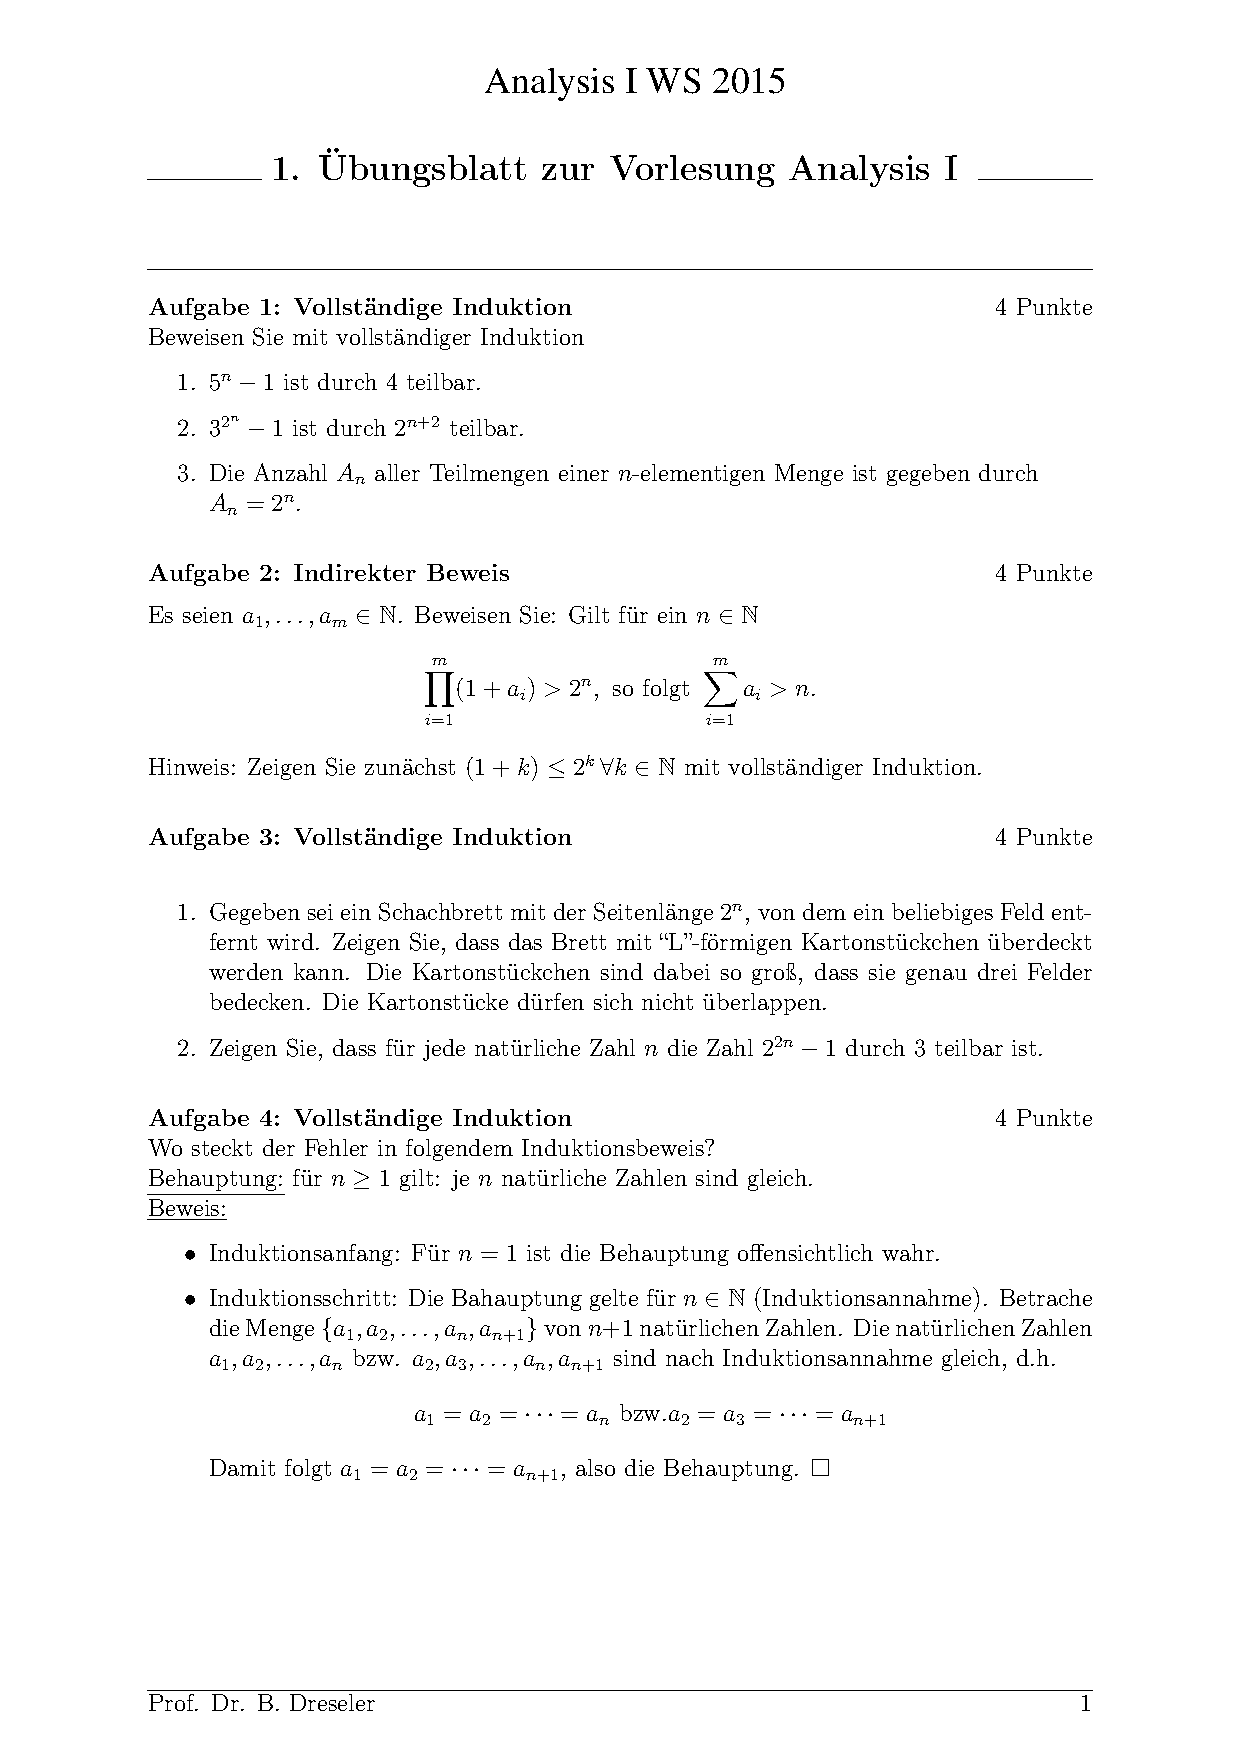
\includepdf[pages=-]{blatt1}
	\section{Übungsblatt 2}\label{uebungsblatt2}
	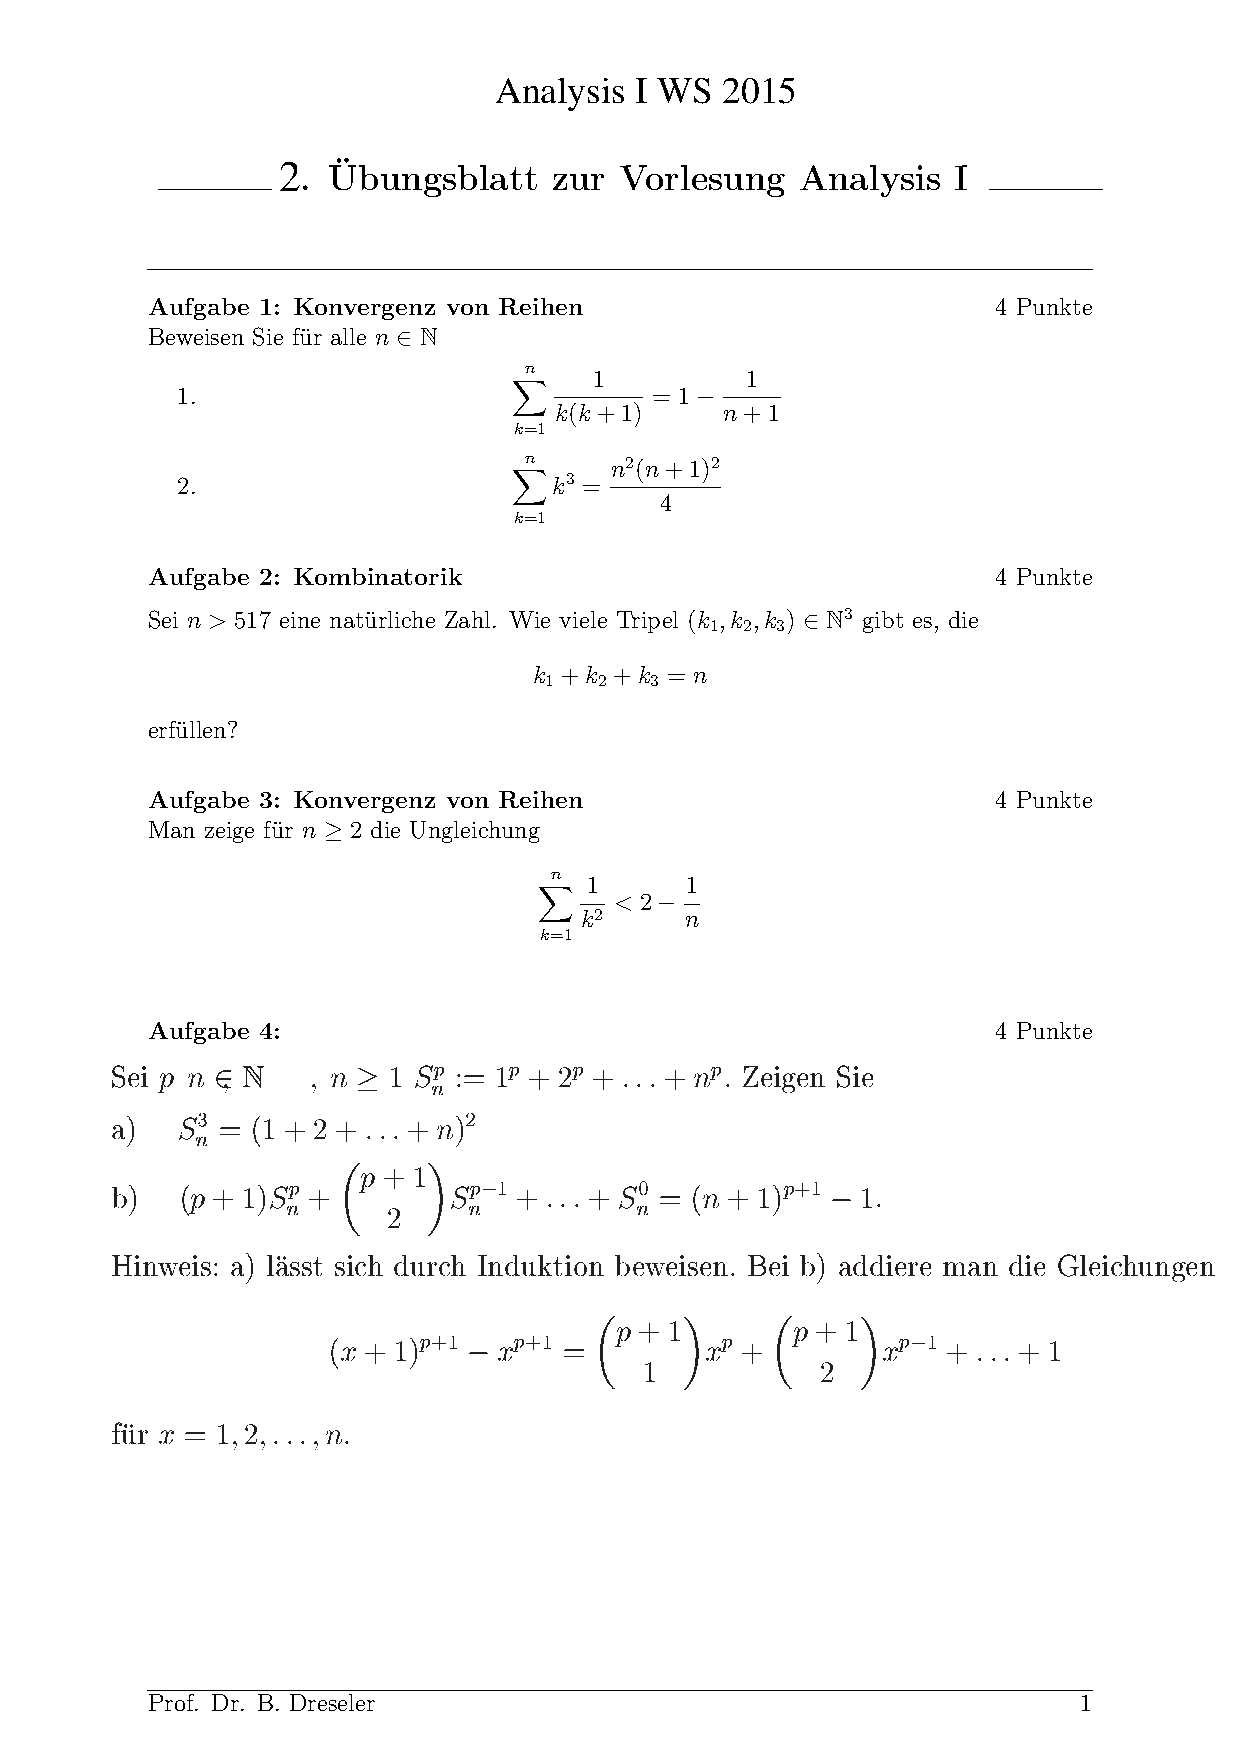
\includepdf[pages=-]{blatt2}
	\section{Übungsblatt 3}\label{uebungsblatt3}
	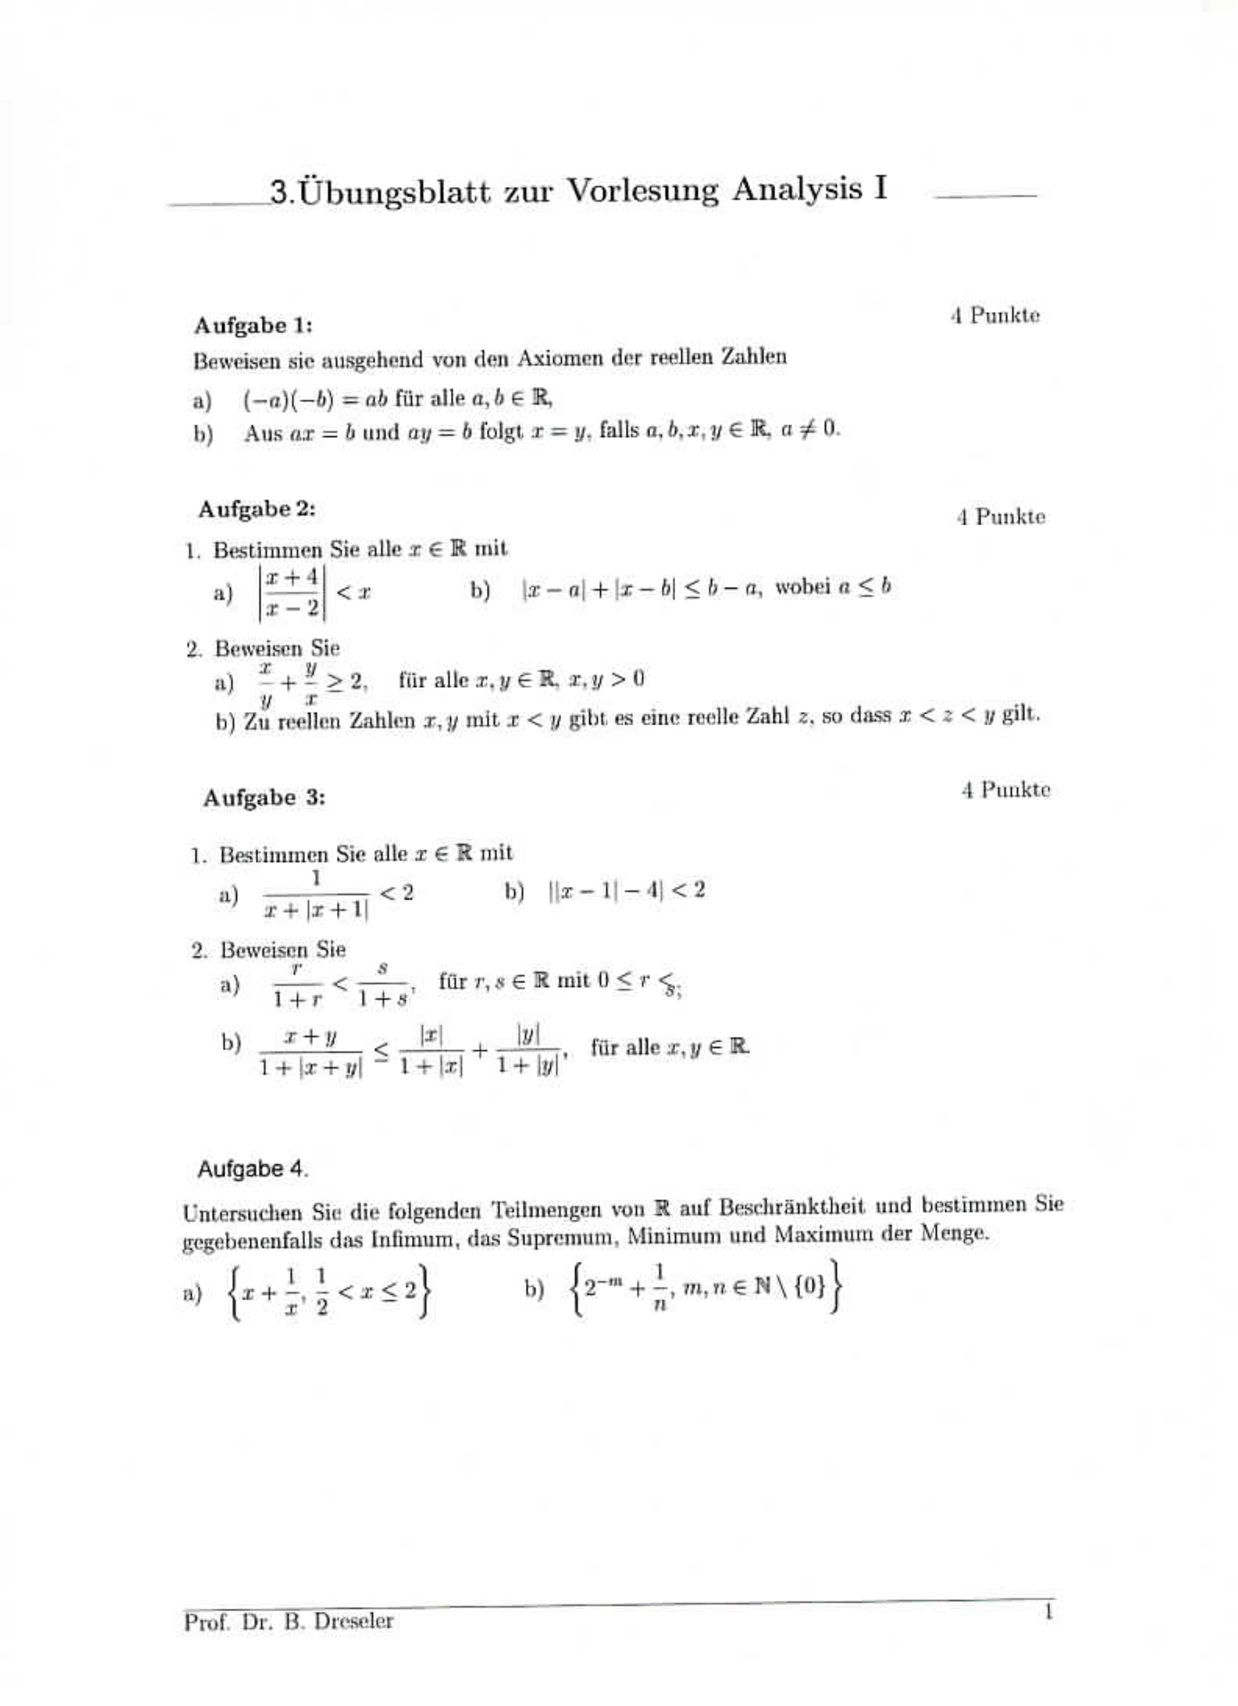
\includepdf[pages=-]{blatt3}
\end{document}